% 8
\subsection{最大生成掌}

\subsubsection{SOJ\,Programming\,Contest\,\texttt\#3\,A}

\frame {
	给定\textsl{带权完全图} $G = (V, E)$,其中 $V = \left\{ 1, 2, \ldots, n \right\}$,边 $(i, j)$ 的权值为 $\abs {i - j}$,\!求 $G$ 的\emm{\slshape 最大生成 \upshape(\slshape 简单\upshape) \slshape 仙人掌}的边权和,\break 并给出一组构造。

	{\color{fuchsia}$1 \leq n \leq 5 \times 10^5$。}
}

\sol {
	\begin{theoe}
		\vspace{-4pt}\hspace{2em}存在一组最优解,满足对于每条桥边 $(u, v)$,均有 $u = 1$ 或 $v = n$。
	\end{theoe}\pause
	\begin{theoe}
		\vspace{-4pt}\hspace{2em}存在一组最优解,不包含长度 $\geq 5$ 的圈。
	\end{theoe}\pause
	\begin{theoe}
		\vspace{-4pt}\hspace{2em}存在一组最优解,每个圈都包含点 $1$ \emm{或}点 $n$。
	\end{theoe}
}

\sol {
	现在允许的构建``材料'':\textsl{桥边}、\textsl{3 元环},\textsl{4 元环}。\pause
	\begin{itemize}
		\item 桥边:桥边只可能形如 $(1, x)$ 或 $(x, n)$,且当 $x \leq n/2$ 时为后者,否则为前者。\pause
		\item 3 元环:3 元环 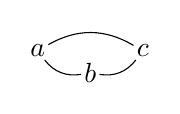
\begin{tikzpicture}[baseline=-1.5pt]
			\path[anchor=base, inner sep=1pt] node (A) at (-0.6667, 0) {$a$} node (B) at (0, -0.3333) {$b$} node (C) at (0.6667, 0) {$c$};
			\draw (A) edge[bend right] (B) edge[bend left] (C) (B) edge[bend right] (C);
		\end{tikzpicture} 对边权和提供 $2 (c - a)$ 的贡献,\textsl{和 $b$ 无关}。\pause
		\item 4 元环:4 元环的摆放形式一定如 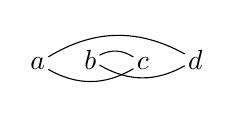
\begin{tikzpicture}[baseline=-1.5pt]
			\path[anchor=base, inner sep=1pt] node (A) at (-1, 0) {$a$} node (B) at (-0.3333, 0) {$b$} node (C) at (0.3333, 0) {$c$} node (D) at (1, 0) {$d$};
			\draw (A) edge[bend right] (C) edge[bend left] (D) (B) edge[bend left] (C) edge[bend right] (D);
		\end{tikzpicture},对边权和可以提供 $2 (c + d - a - b)$ 的贡献。
	\end{itemize}
}

\sol {
	考虑固定使用的圈的个数 $C$。容易发现桥边的优先级是最低的,因此我们先加入圈。这些圈一定可以按照 $\left( 1, n \right), \left( 1, n - 1 \right), \break \left( 2, n \right), \left( 1, n - 2 \right), \left( 3, n \right), \ldots$ 的顺序添加。\pause

	然后剩下的点先加入到对应的 4 元环提供 $2 (r - l)$ 的贡献,然后加入桥边,最后的点留给 3 元环当 $b$ {\footnotesize(``工具人'')}。\pause

	枚举圈的个数 $C$ 即可,时间复杂度 $O(n)$。\pause

	{\footnotesize\color{gray}\sout{当然如果你打表技术高超可以发现答案及构造以\ $9$ 为周期循环的(}}
}

% 9
\subsection{Evil}

\subsubsection{Codeforces\,Round \texttt\#192\,E (Codeforces 329\,E)}

\frame {
	坐标平面上有 $n$ 个互不相同的点 $p_i = (x_i, y_i)$,定义\textsl{带权完全图} $G = (V, E)$,其中 $V = \{p_1, p_2, \ldots, p_n\}$,两点之间的权值为其 Manhattan 距离。求 $G$ 的\emm{\textsl{最长 Hamilton 圈}}的长度。

	{\color{fuchsia}$3 \leq n \leq 10^5$。}
}

\newcommand\valley{{\color{fuchsia}谷}}
\newcommand\peak{{\color{blue}峰}}
\newcommand\flatt{{\color{properpurple}坡}}

\sol {
	先考虑一维的情形,设点的坐标分别为 $x_1 < x_2 < \cdots < x_n$。\pause

	\begin{figure}[htb]
		\begin{minipage}[t]{.494\linewidth}
			\centering
			\begin{tikzpicture}[x=.75cm, y=.75cm, remember picture]
				\useasboundingbox (1, -1.6) rectangle (6, 0.7);
				\draw (1, -0.6) -- (4, -0.6) arc[radius=0.1, start angle=90, delta angle=-180]
								-- (2, -0.8) arc[radius=0.1, start angle=90, delta angle=180]
								-- (5, -1.0) arc[radius=0.1, start angle=90, delta angle=-180]
								-- (3, -1.2) arc[radius=0.1, start angle=90, delta angle=180]
								-- (6, -1.4) arc[radius=0.1, start angle=90, delta angle=-180]
								-- (1, -1.6) arc[radius=0.5, start angle=-90, delta angle=-180];
				\foreach \x in {1,...,6} {
					\draw[dashed] (\x, -1.65) -- (\x, -0.35);
					\node at (\x, 0) {\footnotesize $x_\x$};
				}
				\only<3->{
					\draw[semithick, fuchsia]
						(2.1, -0.8) -- (2, -0.8) arc[radius=0.1, start angle=90, delta angle=180] -- (2.1, -1)
						(3.1, -1.2) -- (3, -1.2) arc[radius=0.1, start angle=90, delta angle=180] -- (3.1, -1.4)
						(1.5, -1.6) -- (1, -1.6) arc[radius=0.5, start angle=-90, delta angle=-180] -- (1.5, -0.6);
					\node[circle] (valley) at (3.5, -4.5) {\valley};
					\draw[gray, <-] (valley) edge (1.1, -1.7) edge (2.1, -1.1) edge (3.1, -1.5);
				}
				\only<4->{
					\draw[semithick, blue]
						(3.9, -0.6) -- (4, -0.6) arc[radius=0.1, start angle=90, delta angle=-180] -- (3.9, -0.8)
						(4.9, -1.0) -- (5, -1.0) arc[radius=0.1, start angle=90, delta angle=-180] -- (4.9, -1.2)
						(5.9, -1.4) -- (6, -1.4) arc[radius=0.1, start angle=90, delta angle=-180] -- (5.9, -1.6);
					\coordinate (jkmx@re@1) at (4.1, -0.9);
					\coordinate (jkmx@re@2) at (5.1, -1.3);
					\coordinate (jkmx@re@3) at (6.1, -1.7);
				}
				\only<6->{
					\draw node at (1, 0.6) {\valley} node at (2, 0.6) {\valley} node at (3, 0.6) {\valley}
						node at (4, 0.6) {\peak} node at (5, 0.6) {\peak} node at (6, 0.6) {\peak};
				}
			\end{tikzpicture}
			\caption{$n$ 是偶数}
		\end{minipage}
		\begin{minipage}[t]{.494\linewidth}
			\centering
			\begin{tikzpicture}[x=.75cm, y=.75cm, remember picture]
				\useasboundingbox (1, -1.6) rectangle (7, 0.7);
				\draw (1, -0.6) -- (5, -0.6) arc[radius=0.1, start angle=90, delta angle=-180]
								-- (2, -0.8) arc[radius=0.1, start angle=90, delta angle=180]
								-- (6, -1.0) arc[radius=0.1, start angle=90, delta angle=-180]
								-- (3, -1.2) arc[radius=0.1, start angle=90, delta angle=180]
								-- (7, -1.4) arc[radius=0.1, start angle=90, delta angle=-180]
								-- (1, -1.6) arc[radius=0.5, start angle=-90, delta angle=-180];
				\foreach \x in {1,...,7} {
					\draw[dashed] (\x, -1.65) -- (\x, -0.35);
					\node at (\x, 0) {\footnotesize $x_\x$};
				}
				\only<3->{
					\draw[semithick, fuchsia]
						(2.1, -0.8) -- (2, -0.8) arc[radius=0.1, start angle=90, delta angle=180] -- (2.1, -1)
						(3.1, -1.2) -- (3, -1.2) arc[radius=0.1, start angle=90, delta angle=180] -- (3.1, -1.4)
						(1.5, -1.6) -- (1, -1.6) arc[radius=0.5, start angle=-90, delta angle=-180] -- (1.5, -0.6);
					\draw[gray, <-] (valley) edge (0.4, -1.2) edge (1.9, -1.1) edge (2.9, -1.5);
				}
				\only<4->{
					\draw[semithick, blue]
						(4.9, -0.6) -- (5, -0.6) arc[radius=0.1, start angle=90, delta angle=-180] -- (4.9, -0.8)
						(5.9, -1.0) -- (6, -1.0) arc[radius=0.1, start angle=90, delta angle=-180] -- (5.9, -1.2)
						(6.9, -1.4) -- (7, -1.4) arc[radius=0.1, start angle=90, delta angle=-180] -- (6.9, -1.6);
					\node[circle] (peak) at (3.5, -4.5) {\peak};
					\draw[gray, <-] (peak) edge (4.9, -0.9) edge (5.9, -1.3) edge (6.9, -1.7)
										   edge (jkmx@re@1) edge (jkmx@re@2) edge (jkmx@re@3);
				}
				\only<5->{
					\draw[thick, properpurple] (3.833, -1) -- (4.167, -1);
					\node[circle] (flat) at ($(valley)!0.5!(peak)$) {\flatt};
					\draw[gray, <-] (flat) edge (3.9, -1.1);
				}
				\only<6->{
					\draw node at (1, 0.6) {\valley} node at (2, 0.6) {\valley} node at (3, 0.6) {\valley}
						node at (4, 0.6) {\flatt} node at (5, 0.6) {\peak} node at (6, 0.6) {\peak} node at (7, 0.6) {\peak};
				}
			\end{tikzpicture}
			\caption{$n$ 是奇数}
		\end{minipage}
	\end{figure}
}

\sol {
	\begin{theoe}
		\vspace{-4pt}\hspace{2em}\valley 的数量等于\peak 的数量。
	\end{theoe}\pause
	\begin{theoe}
		\vspace{-4pt}\hspace{2em}\valley\peak\flatt 序列可以确定答案。具体地,\valley 的贡献为 $-2$,\peak 的贡献为 $2$,\flatt 的贡献为 $0$。
	\end{theoe}
}

\sol {
	\begin{theoe}[最大值的条件]
		\vspace{-4pt}\hspace{2em}在一维情形下,最大值取到当且仅当前$\left\lfloor \frac n2 \right\rfloor$个元素均为\valley,后$\left\lfloor \frac n2 \right\rfloor$个元素均为\peak。
	\end{theoe}\pause
	\begin{theoe}[\valley\peak\flatt 序列的可行性]
		\vspace{-4pt}\hspace{2em}一个\valley\peak\flatt 序列是可行的,当且仅当 $1$ 是\valley,$n$ 是\peak,且去掉所有的\flatt 后,\!$2 \sim n - 1$ 构成一个合法括号序列,\!其中视\valley 为\kern0pt{\upshape\color{fuchsia}\texttt(},\break 视\peak 为 {\upshape\color{blue}\texttt)}。
	\end{theoe}
}

\sol {
	什么时候取次大值?\pause
	\begin{itemize}
		\item $n = 2 k$ 为偶数:$\underbrace{\text{\valley\valley}\ldots\text\valley}_{k-1}\text{\flatt\flatt}\underbrace{\text{\peak\peak}\ldots\text\peak}_{k-1}$。\pause
		\item $n = 2 k + 1$ 为奇数:此时有两种情形:$\underbrace{\text{\valley\valley}\ldots\text\valley}_k\text{\peak\flatt}\underbrace{\text{\peak\peak}\ldots\text\peak}_{k-1}$ 和 $\underbrace{\text{\valley\valley}\ldots\text\valley}_{k-1}\text{\flatt\valley}\underbrace{\text{\peak\peak}\ldots\text\peak}_k$。
	\end{itemize}\pause

	那这个条件有多\textsl{宽}呢?
}

\sol {
	\begin{theoe}[$n$ 为偶数时的次大值可行定理]
		\vspace{-4pt}\hspace{2em}设 $n = 2 k$ 为偶数。若我们给 $x_1, x_2, \ldots, x_n$ \emm{任意黑白染色}(黑白点各 $k$ 个),并要求排列必须是黑白交替的形式。不妨设 $x_1$ 是白点,则
		\begin{itemize}
			\divide\itemsep4%
			\item 当所有白点都在黑点左边时,可以取到最大值。
			\item 否则,\emm{一定能取到次大值}。
		\end{itemize}
	\end{theoe}
}

\sol {\vspace{16pt}
	\begin{theoe}[$n$ 为奇数时的次大值可行定理]
		\vspace{-4pt}\hspace{2em}设 $n = 2 k + 1$ 为奇数。若我们给 $x_1, x_2, \ldots, x_n$ 中的其中 $2 k$ 个点黑白染色 (黑白点各 $k$ 个),并要求同色点不能相邻。不妨设 $x_1$ 是白点,则
		\begin{itemize}
			\divide\itemsep4%
			\item 若中间点 $x_{k+1}$ 未被染色,且所有白点都在黑点左边时,可以取到最大值。
			\item 中间点 $x_{k+1}$ 未被染色的其余情况均可取到任意一种次大值。
			\item 若中间点 $x_{k+1}$ 被染色,则一定能取到\emm{\textsl{最大}}值。
		\end{itemize}
	\end{theoe}\pause

	综上,最优方案只可能是下列三者之一:($x$ 最大, $y$ 最大)、($x$ 最大, $y$ 次大)、($x$ 次大, $y$ 最大)。时间复杂度为排序后线性。
}

% 10
\subsection{Jeopardy}

\subsubsection{ByteDance\,Moscow\,Workshops\,Camp\,2022\,Online\,Contest\,J}

\frame {
	考虑完全图 $K_{16} = (V, E)$,其中 $V = \left\{ 1, 2, \ldots, 16 \right\}$,你需要将 $E$ 划分成 $20$ 个大小为 $6$ 的子集,使得每个子集是某个 $K_4$ 的 $6$ 条边 (即 $K_{16}$ 的边 $K_4$ 划分)。

	进一步,其中某些子集是预先给出的,即你的划分中必须完整地包含这些子集。请给出一组构造或说明无解。
}

\sol {\vspace{8pt}
	这其实是一个 Steiner 系 $\mathsf S(2, 4, 16)$ 问题。先考虑\emm{\textsl{没有预先给出子集时}}如何直接构造。\pause

	考虑有限域 $\f F_4 \!=\! \{0, 1, \i, \i \!+\! 1\}$ 上的所有直线 $a x \!+\! b y \!+\! c \!=\! 0$。由于两点确定一条直线,两条直线不会有多于一个交点。\pause

	\begin{figure}[htb]
		\centering
		\begin{tikzpicture}[x=.6cm, y=.6cm]
			\useasboundingbox (-1, -0.5) rectangle (3, 3);
			\fill[nearly opaque, white] (-1.6, -0.85) rectangle (3.5, 3.5);
			\begin{scope}[circle, minimum size=2pt]
				\node foreach \x in {0,...,3} foreach \y in {0,...,3} [fill] at (\x, \y) {};
			\end{scope}
			\begin{scope}[inner sep=5pt]
				\draw[below]node at (0, 0) {\footnotesize $0$}
							node at (1, 0) {\footnotesize $1$}
							node at (2, 0) {\footnotesize $\i$}
							node at (3, 0) {\footnotesize $\i + 1$};
				\draw[left] node at (0, 0) {\footnotesize $0$}
							node at (0, 1) {\footnotesize $1$}
							node at (0, 2) {\footnotesize $\i$}
							node at (0, 3) {\footnotesize $\i + 1$};
			\end{scope}
			\draw[semithick, fuchsia] (-0.1, 2.573) .. controls (0.941667, -3.996444) and (1.983333, 8.639840) .. (3.025, -0.20825);
		\end{tikzpicture}
		\caption{直线 $x + \i y + (\i + 1) = 0$}
	\end{figure}

	\vspace{-12pt}\pause
	直线斜率一共有 $0, 1, \i, \i + 1, \infty$ 共 $5$ 种,每种直线有 $4$ 条,这样就是一个可行的构造。
}

\sol {
	\begin{theoe}
		\vspace{-4pt}\hspace{2em}所有的 Steiner 系 $\mathsf S(2, 4, 16)$ 都是同构的。
	\end{theoe}\pause

	于是任意一组解 (如果存在的话),一定可以通过仿射变换变成标准解。于是任意找两个有公共点的边子集,规定其中一条为 $x$ 轴 ($y = 0$),其中一条为 $y$ 轴 ($x = 0$),剩余情况枚举排列验证。\pause

	时间复杂度 $3 ! \cdot 9 ! \cdot \textit{验证时间}$。
}

% 11
\subsection{GCD Land}

\subsubsection{CCPC\,Final\,2018\,C (Codeforces\,Gym 102055\,C)}

\frame {
	给定图 $G = (V, E)$,其中 $V = \f N, E = \bigl\{ (i, j) \bigm\arrowvert \text{$i, j \in \f N$ 且} \break \gcd(i, j) \mathbin> 1 \bigr\}$。给定 $N$,求是否存在 $X \mathbin\in \f N$ 满足 $S_X \mathbin= \{X, X + 1, \break \ldots, X \!+\! N \!-\! 1\}${\def\ {\hspace{2.6pt plus 3pt minus 3pt}}\ 导出的子图\ $G[S_X]$\ 连通,\!若是,\!给出满足条件的\ $X$。\!\!}

	{\color{fuchsia}$1 \leq N \leq 10^5$。}
}

\sol {
	不妨设 $N$ 足够大。若取 $M = \prod\limits_{p \leq n, p \in \f P} p$,则对于任意 $x \in [-n, n] \setminus \{\pm 1\}$,$M$ 和 $M + x$ 之间连有边。

	\begin{figure}[htb]
		\centerline{
		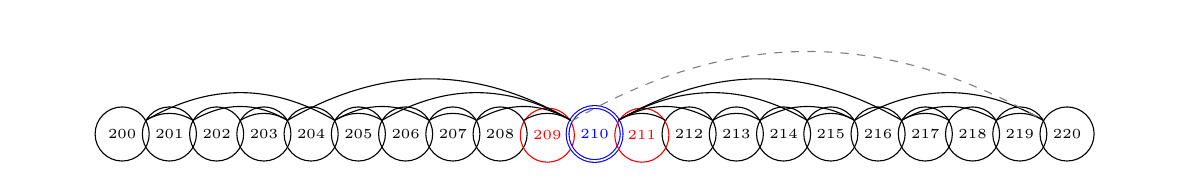
\begin{tikzpicture}[x=.6cm, y=.6cm]
			\fill[nearly opaque, white] (-12, -0.5) rectangle (12, 2);
			\begin{scope}[circle]
				\node foreach \x in {-10,...,-2,2,3,...,10} [draw] (\x) at (\x, 0) {\tiny $\the\numexpr\x+210$};
				\node[draw, red] (-1) at (-1, -0.025) {\tiny $209$};
				\node[draw, double, blue] (0) at (0, 0) {\tiny $210$};
				\node[draw, red] ( 1) at ( 1, -0.025) {\tiny $211$};
			\end{scope}
			\draw[bend left]
				(-10) edge (-8) (-8) edge (-6) (-6) edge (-4) (-4) edge (-2) (-2) edge (0) (0) edge (2) (2) edge (4) (4) edge (6) (6) edge (8) (8) edge (10)
				(-9) edge (-6) (-6) edge (-3) (-3) edge (0) (0) edge (3) (3) edge (6) (6) edge (9)
				(-10) edge (-5) (-5) edge (0) (0) edge (5) (5) edge (10)
				(-7) edge (0) (0) edge (7)
				(-1) edge[dashed, gray] (10);
		\end{tikzpicture}
		}
		\caption{}
	\end{figure}

	\vspace{-24pt}\pause
	也就是说,这 $2 n + 1$ 个点几乎是连通的——除了 $M \pm 1$。
}

\sol {\vspace{8pt}
	如何将 $M \pm 1$ 连上?``借用''小素数。
	\begin{figure}[htb]
		\centering
		\begin{tikzpicture}[x=.666667cm, y=.666667cm]
			\useasboundingbox (-7.25, -4.25) rectangle (7.25, 2.5);
			\fill[nearly opaque, white] (-7.25, -5.25) rectangle (7.25, 2.5);
			\draw (-4, 1) -- (4, 1) (-4, 0) -- (4, 0);
			\draw foreach \x in {-3,...,3} {(\x, 0) -- +(0, 1)};
			\draw[<-] (-1, 1.25) -- +(0, 0.75) node [above, inner sep=3pt] {$n$};
			\fill[nearly transparent, fuchsia]	(-3, 0) rectangle +(1, 1);
			\fill[nearly transparent, blue]		(-2, 0) rectangle +(1, 1);
			\fill[nearly transparent, orange]	(-1, 0) rectangle +(1, 1);
			\fill[nearly transparent, aqua]		( 0, 0) rectangle +(1, 1);
			\fill[nearly transparent, properpink](1, 0) rectangle +(1, 1);
			\fill[nearly transparent, yellow]	( 2, 0) rectangle +(1, 1);
			\path node at (-3.45, 0.5) {$\cdots$} node at (-2.5, 0.5) {$p_1$} node at (-1.5, 0.5) {$p_2$} node at (-0.5, 0.5) {$q_1$}
				node at (0.5, 0.5) {$q_2$} node at (1.5, 0.5) {$q_3$} node at (2.5, 0.5) {$q_4$} node at (3.55, 0.5) {$\cdots$} node at (-6, 0.5) {\footnotesize 素数表 (<):};
			% graph
			\draw (-7.5, -2) -- (7.5, -2) (-7.5, -3) -- (7.5, -3);
			\draw foreach \x in {0.5,1.5,3.9,4.9,5.2,6.2,6.5,7.5} {(-\x, -3) -- +(0, 1) (\x, -3) -- +(0, 1)};
			\path
				node at (-7, -2.5) {\scriptsize $M\!\!-\!\!n$}
				node at (-5.7, -2.5) {\scriptsize $M\!\!-\!\!p_2$}
				node at (-4.4, -2.5) {\scriptsize $M\!\!-\!\!p_1$}
				node at (-1, -2.5) {\scriptsize $M\!\!-\!\!1$}
				node at (0, -2.5) {\scriptsize $M$}
				node at (1, -2.5) {\scriptsize $M\!\!+\!\!1$}
				node at (4.4, -2.5) {\scriptsize $M\!\!+\!\!p_1$}
				node at (5.7, -2.5) {\scriptsize $M\!\!+\!\!p_2$}
				node at (7, -2.5) {\scriptsize $M\!\!+\!\!n$}
				node at (-2.7, -1.7) {$\cdots$}
				node at (2.7, -1.7) {$\cdots$};
			\draw[dashed, bend right] (0, -2) edge +(-2, 0.2) edge +(-7, 0.2);
			\draw[dashed, bend left] (0, -2) edge +(2, 0.2) edge +(7, 0.2);

			\only<1>{
				\fill[nearly transparent, red] (-1.5, -3) rectangle +(1, 1);
				\fill[nearly transparent, fuchsia] (-4.9, -3) rectangle +(1, 1) (3.9, -3) rectangle +(1, 1);
				\draw[semithick, fuchsia] (0, -2)
					edge[->, bend right, "\scriptsize $p_1$"{very near end, below right}] +(-4.4, 0)
					edge[->, bend left,  "\scriptsize $p_1$"{very near end, below left}]  +(4.4, 0);
			}
			\only<1-2>{
				\fill[nearly transparent, red] (0.5, -3) rectangle +(1, 1);
				\fill[nearly transparent, blue] (-6.2, -3) rectangle +(1, 1) (5.2, -3) rectangle +(1, 1);
				\draw[semithick, blue] (0, -2)
					edge[->, bend right, "\scriptsize $p_2$"{very near end, below right}] +(-5.7, 0)
					edge[->, bend left,  "\scriptsize $p_2$"{very near end, below left}]  +(5.7, 0);
			}
			\only<2-3>{
				\fill[nearly transparent, red] (-4.9, -3) rectangle +(1, 1);
			}
			\only<2-4>{
				\fill[nearly transparent, red] (3.9, -3) rectangle +(1, 1);
			}
			\only<3-5>{
				\fill[nearly transparent, red] (-6.2, -3) rectangle +(1, 1);
			}
			\only<3-6>{
				\fill[nearly transparent, red] (5.2, -3) rectangle +(1, 1);
			}
			% steps
			\only<2->{
				\fill[nearly transparent, fuchsia] (-1.5, -3) rectangle +(1, 1);
				\draw[bend right] (-1, -3) edge[->, semithick, fuchsia, "\scriptsize $p_1$"{below=1pt}] +(4.4, -0.2);
			}
			\only<3->{
				\fill[nearly transparent, blue] (0.5, -3) rectangle +(1, 1);
				\draw[bend left] (1, -3) edge[->, semithick, blue, "\scriptsize $p_2$"{below=1pt}] +(-5.7, -0.2);
			}

			\only<4->{
				\fill[nearly transparent, orange] (-4.9, -3) rectangle +(1, 1);
				\draw[bend left] (-4.4, -2) edge[->, semithick, orange, "\scriptsize $q_1$"{above=1pt}] +(6.8, 0.2);
			}
			\only<5->{
				\fill[nearly transparent, aqua] (3.9, -3) rectangle +(1, 1);
				\draw[bend right] (4.4, -2) edge[->, semithick, aqua, "\scriptsize $q_2$"{above=1pt}] +(-7.2, 0.2);
			}
			\only<6->{
				\fill[nearly transparent, properpink] (-6.2, -3) rectangle +(1, 1);
				\draw[bend right] (-5.7, -3) edge[->, semithick, properpink!75!black, "\scriptsize $q_3$"{below=1pt}] +(8.4, -0.2);
			}
			\only<7->{
				\fill[nearly transparent, yellow] (5.2, -3) rectangle +(1, 1);
				\draw[bend left] (5.7, -3) edge[->, semithick, yellow!75!black, "\scriptsize $q_4$"{below=1pt}] +(-9, -0.2);
			}
		\end{tikzpicture}
	\end{figure}

	\onslide<8->{只需 $q_2 \leq p_1 + n, \ q_4 \leq p_2 + n\only<9->{\;\Leftarrow\; n \geq 19}$。}
}

\sol {\vspace{4pt}
	当 $N \geq 39$ 时,{\footnotesize\vspace{-8pt}\[ \begin{cases} M \equiv 1 &\pmod {p_1} \\ M \equiv -1 &\pmod {p_2} \\ M \equiv p_1 &\pmod {q_1} \\ M \equiv - p_1 &\pmod {q_2} \\ M \equiv p_2 &\pmod {q_3} \\ M \equiv - p_2 &\pmod {q_4} \end{cases} \]}

	\vspace{-4pt}\pause
	对小于 $p_1$ 的素数 $p$,我们要求 $p \mid M$,使用 CRT 即可找到符合要求的 $M$。\pause

	当 $17 \mathbin\leq N \mathbin< 39$ 时,\!暴力枚举,\!最小解不超过 $10^7$。\!否则无解。
}

% 12
\subsection{City}

\subsubsection{JOISC\,2017 D4T2}

\frame {\vspace{12pt}
	{\footnotesize\color{gray} 这是一道通信题。}

	给定一棵 $N$ 个顶点的有根树,保证所有顶点的深度 (到根的距离) 不超过 $18$。Alice 需要给每个顶点 $v$ 进行编码 $c_v$,需要满足 $0 \leq c_v \leq 2^{28} - 1$。

	Bob 不知道关于这棵树的任何信息,而 Bob 需要回答若干次询问:每次询问 Bob 将收到顶点 $x, y$ ($x \neq y$) 的\emm{\textsl{编码}}\ $c_x, c_y$,然后 Bob 需要判断以下三种情况哪一种成立:
	\begin{enumerate}
		\setcounter{enumi}{-1}\divide\itemsep3%
		\item $y$ 是 $x$ 的祖先。
		\item $x$ 是 $y$ 的祖先。
		\item $x, y$ 不存在祖先关系。
	\end{enumerate}

	{\color{fuchsia}$2 \leq N \leq 2.5 \times 10^5$。}
}

\sol {
	如何判定祖先关系?dfs 序。\pause

	{\def\ {\hspace{3pt plus 3pt minus 3pt}}设顶点\ $v$\ 的\ dfs\ 时间戳为\ $i_v$\ (即\ $v$\ 是\ dfs\ 序中的第\ $i_v$\ 个顶点),\ }\break 以 $v$ 为根的子树中时间戳最大者为 $e_v$ (即搜完这棵子树时的总点数),则 \[ \text{$u$ 是 $v$ 的祖先} \iff \text{$i_u \leq i_v \leq e_u$}. \]

	\pause 令 $c_v = (i_v, e_v)$ 即可完成,但是传输信息量为 $2 \log_2 N \approx\break \unit{36}\bit > \unit{28}\bit$。
}

\sol {\vspace{8pt}
	\def\hzk{\genfrac{}{}{0pt}0}
	$i_u \leq i_v \leq e_u \iff 0 \leq i_v - i_u \leq \only<2->{\color{fuchsia}} e_u - i_u$。

	\vspace{4pt}\hskip151pt\onslide<2->{$\hzk \Downarrow {\only<3->{\llap{$0 \leq i_v - i_u \leq {}$}} \color{blue} \mathit{size}_u - 1}$}

	\vspace{8pt}
	\onslide<4->{令 $c_v = (i_v, \mathit{size}_v)$,同样可以完成目的,但最坏情况下传输信息量仍为 $2 \log_2 N$。}

	\onslide<5->{\emm{\textsl{保证所有顶点的深度不超过 $18$。}}}\onslide<6->{$\sum\limits_v \mathit{dep}_v \leq 18 N$。}

	\vspace{-4pt}
	\onslide<7->{\[ \sum_v \mathit{size}_v = \sum_v (\mathit{dep}_v + 1) \onslide<8->{\leq 19 N = O(N) \ \color{gray} !} \]}

	\vspace{-8pt}
	\onslide<9->{$\mathit{size}_v$ 的种数不会很多。然而 Bob 无法得知是哪些值。}

	\onslide<10->{通过加入虚点固定 $\mathit{size}_v$ 的可能取值!}
}

\sol {\vspace{8pt}
	常见的技巧:向\textsl{等比数列}拟合。\pause

	\begin{figure}[htb]
		\centering
		\begin{tikzpicture}[x=.75cm, y=.75cm]
			\fill[nearly opaque, white] (-5, -0.7) rectangle (5, 1);
			\draw (-4.5, 1) -- (4.5, 1) (-4.5, 0) -- (4.5, 0);
			\foreach \x/\y in {-4/q^i, -3.410182/q^{i+1}, -2.628839/q^{i+2}, -1.593781/q^{i+3}, -0.222620/q^{i+4}, 1.593781/q^{i+5}, 4/q^{i+6}} {
				\draw (\x, 0) -- +(0, 1);
				\node at (\x, -0.3) {\footnotesize $\y$};
			}
			\begin{scope}[->, fuchsia, circle, minimum size=2.5pt, every node/.style=fill]
				\draw (-3, 0.5) node {} -- (-2.628839, 0.5);
				\draw (-2, 0.5) node {} -- (-1.593781, 0.5);
				\draw (-1, 0.5) node {} -- (-0.222620, 0.5);
				\draw (0.3, 0.6) node {} -- (1.593781, 0.6);
				\draw (1, 0.4) node {} -- (1.593781, 0.4);
				\draw (2.5, 0.5) node {} -- (4, 0.5);
			\end{scope}
		\end{tikzpicture}
		\caption{}
	\end{figure}

	\vspace{-12pt}
	考虑等比数列 $\{ q^n \} = \left\{ 1, q, q^2, q^3, \ldots \right\}$ ($q > 1$),然后将每个 $\mathit{size}_v$ 取到不小于 $\mathit{size}_v$ 的最小 $q^k$。\pause

	分析可知,最终的总点数不会超过\vspace{-4pt}\[ \sum_v q^{\mathit{dep}_v} \leq q^{18} N. \]
}

\sol {
	经如此量化后,\!不同的 $\mathit{size}_v$ 的可能取值约为 $\log_q \bigl( q^{18} N \bigr)$ 种。\pause

	最终的传输信息量不超过\vspace{-8pt}\[ \left\lceil \log_2 \Bigl( \log_q \bigl( q^{18} N \bigr) \Bigr) \right\rceil + \left\lceil \log_2 \bigl( q^{18} N \bigr) \right\rceil \enskip \bit, \]

	\pause\vspace{-6pt}\noindent 取 $q = 1.06$ 可知其不超过 $28$。
}

% 13
\subsection{大鱼划水}

\subsubsection{2020--2021 集训队作业 (loj\,3392)}

\frame {
	坐标平面上有 $n$ 个互不相同的点 $(x_i, y_i)$,你需要在每个点上写一个 $1 \sim n$ 之间的整数,并保证这些整数互不相同。

	定义一条直线为``好的'',如果它满足如下三个条件:
	\begin{itemize}
		\item 平行于坐标轴 ($x$ 轴或 $y$ 轴);
		\item 经过至少一个 (给定的) 点;
		\item 经过的所有点上所写的数的最大公约数为 $1$。
	\end{itemize}

	求``好的''直线的数量的最大值,并给出一组构造。

	{\color{fuchsia}$1 \leq n \leq 2 \times 10^5$。}
}

\sol {
	建立二分图模型,离散化坐标后,对每一条 (经过点的) 水平线 ($x = x_0$) 及竖直线 ($y = y_0$) 建立一个顶点,然后对于题目中的点 $(x_i, y_i)$,我们可以将其看成连接 $x_i$ 和	$y_i$ 的一条\textsl{权值为所写的数}的边,从而得到二分图 $G = (V, E)$,其中 $\abs E = n$。\pause

	一条直线是``好的'',当且仅当其在 $G$ 中对应的点 $v$,所关联的所有边的权值的 $\gcd$ 为 $1$。称这样的点为\emm{\textsl{互素}}的。\pause

	问题转化为最大化\textsl{互素}顶点的个数。
}

\sol {
	考虑答案的上界。\pause

	如果一个顶点 $v$ 的度数 $d(v) = 1$,那么 $v$ 是\textsl{互素}的当且仅当与之关联的唯一边权值为 $1$。\pause

	因此,设 $G$ 中有 $k$ 个 1 度点,则:\pause
	\begin{itemize}
		\item 若存在两个 1 度点之间有边相连,\!则答案不超过 $\abs V - k + 2$。\pause
		\item 否则,答案不超过 $\abs V - \max \bigl\{ \abs k - 1, 0 \bigr\}$。
	\end{itemize}\pause

	实践表明,这个上界很可能就是紧的,因此下面考虑构造。
}

\sol {\vspace{20pt}
	如何构造互素的整数?\pause\textsl{\color{fuchsia}相邻的正整数一定互素}!\pause

	希望对于每个度数 $\geq 2$ 的点,总有两条出边是相邻的 (即作为路径``经过''这个点)。\pause

	对于 $G$ 是连通图的情形,只要贪心取链即可:

	\begin{figure}[htb]
		\centering
		\begin{tikzpicture}[x=.75cm, y=.75cm]
			\fill[nearly opaque, white] (-2, -5) rectangle (2, 0.5);
			\begin{scope}[circle, minimum size=15pt, text opacity=1, every node/.style=draw]
				\alt<4,11>		{\node[fill=fuchsia, fill opacity=.25]}\node (1) at (0, 0) {1};
				\alt<5,13,16>	{\node[fill=fuchsia, fill opacity=.25]}\node (2) at (-1.5, -1.5) {2};
				\alt<6,10>		{\node[fill=fuchsia, fill opacity=.25]}\node (3) at (0, -1.5) {3};
				\alt<9,12>		{\node[fill=fuchsia, fill opacity=.25]}\node (4) at (1.5, -1.5) {4};
				\alt<7,14>		{\node[fill=fuchsia, fill opacity=.25]}\node (5) at (0, -3) {5};
				\alt<15,17>		{\node[fill=fuchsia, fill opacity=.25]}\node (6) at (-0.75, -4.5) {6};
				\alt<8,18>		{\node[fill=fuchsia, fill opacity=.25]}\node (7) at (0.75, -4.5) {7};
			\end{scope}
			\only<-4> {\path (1) edge (2);}
			\only<-5> {\path (2) edge (3);}
			\only<-6> {\path (3) edge (5);}
			\only<-7> {\path (5) edge (7);}
			\only<-8> {\path (7) edge (4);}
			\only<-9> {\path (4) edge (3);}
			\only<-10>{\path (3) edge (1);}
			\only<-11>{\path (1) edge (4);}
			\only<-13>{\path (2) edge (5);}
			\only<-14>{\path (5) edge (6);}
			\only<-15>{\path (6) edge (2);}
			\only<-17>{\path (6) edge (7);}
			\begin{scope}[->, thick, fuchsia]
				\only<5-12>	{\path (1) edge["\footnotesize 1" '					] (2);}
				\only<6-12>	{\path (2) edge["\footnotesize 2"  {inner sep=1pt}	] (3);}
				\only<7-12>	{\path (3) edge["\footnotesize 3" '{inner sep=1pt}	] (5);}
				\only<8-12>	{\path (5) edge["\footnotesize 4"					] (7);}
				\only<9-12>	{\path (7) edge["\footnotesize 5" '					] (4);}
				\only<10-12>{\path (4) edge["\footnotesize 6" '{inner sep=1pt}	] (3);}
				\only<11-12>{\path (3) edge["\footnotesize 7"  {inner sep=1pt}	] (1);}
				\only<12>	{\path (1) edge["\footnotesize 8"					] (4);}
				\only<14-16>{\path (2) edge["\footnotesize 9" '					] (5);}
				\only<15-16>{\path (5) edge["\footnotesize 10"'					] (6);}
				\only<16>	{\path (6) edge["\footnotesize 11"					] (2);}
				\only<18>	{\path (6) edge["\footnotesize 12"'{inner sep=1pt}	] (7);}
			\end{scope}
			\begin{scope}[semithick, blue]
				\only<13->{
					\path (1) edge["\footnotesize 1" '					] (2);
					\path (2) edge["\footnotesize 2"  {inner sep=1pt}	] (3);
					\path (3) edge["\footnotesize 3" '{inner sep=1pt}	] (5);
					\path (5) edge["\footnotesize 4"					] (7);
					\path (7) edge["\footnotesize 5" '					] (4);
					\path (4) edge["\footnotesize 6" '{inner sep=1pt}	] (3);
					\path (3) edge["\footnotesize 7"  {inner sep=1pt}	] (1);
					\path (1) edge["\footnotesize 8"					] (4);
				}
				\only<17->{
					\path (2) edge["\footnotesize 9" '					] (5);
					\path (5) edge["\footnotesize 10"'					] (6);
					\path (6) edge["\footnotesize 11"					] (2);
				}
				\only<19->{
					\path (6) edge["\footnotesize 12"'{inner sep=1pt}	] (7);
				}
			\end{scope}
			\only<20->{ \path[fuchsia, semithick, angle radius=10pt]
				pic[draw] {angle=3--1--4}
				pic[draw] {angle=3--2--1}
				pic[draw] {angle=4--3--1}
				pic[draw] {angle=3--4--7}
				pic[draw] {angle=7--5--3}
				pic[draw] {angle=5--6--2}
				pic[draw] {angle=4--7--5};
			}
		\end{tikzpicture}
	\end{figure}
}

\sol {
	当 $G$ 不再连通时,这个算法会出什么问题呢?\pause

	唯一的问题在于,当我们对其它连通分量贪心时,\textsl{第一条边}的权值不再是 $1$,这将导致最初的顶点 $v$ 不一定\textsl{互素}。\pause

	但就连通分量而言,当固定区间后,有的连通分量本身就无法完成:如 $3, 4, 5, 6$ 就无法分配给一个长度为 $4$ 的圈使得所有点都\textsl{互素},因为与 $6$ 互素的只有 $5$。\pause

	\compress{-8pt}{不过,\!对于\textsl{非圈的}连通分量\,$G$,\!我们只需简单修改一下该算法。\!}
}

\sol {\vspace{20pt}
	\begin{itemize}
		\item 如果连通分量存在 1 度点,那么显然从它开始。\pause
		\item 否则,该连通分量中一定存在一个圈,且圈中至少有一个点的度数 $\geq 3$,记这个点为 $r$。\pause
	\end{itemize}
	\begin{figure}[htb]
		\centering
		\begin{tikzpicture}[x=.75cm, y=.75cm]
			\useasboundingbox (-2.6, -2.6) rectangle (5.5, 0.25);
			\fill[nearly opaque, white] (-2.6, -2.6) rectangle (5.5, 0.5);
			\begin{scope}[circle, minimum size=15pt]
				\node[draw] (r) at (0, 0) {$r$};
				\node[draw] (v) at (2.5, 0) {$v$};
				\node		(u) at (5.1, 0) {$\cdots$};
			\end{scope}
			\begin{scope}[->, semithick, fuchsia]
				\path (r) edge[out=270, in=180, looseness=24, "\footnotesize $\lambda$"{pos=.9375, inner sep=1pt}] (r) edge["\footnotesize $\lambda + 1$"{inner sep=1pt}] (v);
				\path (v) edge (4.6, 0);
			\end{scope}
		\end{tikzpicture}
		\caption{}
	\end{figure}
}

\sol {
	现在只剩下一类问题:圈。\pause

	我们需要将这些圈作为整体考虑,即假设 $G$ 是由若干个圈构成的 \emm{\textsl{2-正则图}}。\pause

	$G$ 是二分图 $\Rightarrow G$ 只包含偶圈。\pause

	在这个子问题中,点和边的地位是对等的,因此可以考虑给点分配 $1 \sim \abs V$ 的标号,使得相邻点标号互素。\pause

	等价地,令 $H_n = (V_n, E_n)$,其中 $V_n = \{ 1, 2, \ldots, n \}, E_n =\break \left\{ \vbox to9pt{} (i, j) \middle\arrowvert \text{$1 \leq i, j \leq n$ 且 $\gcd(i, j) = 1$} \right\}$。
}

\sol {\vspace{12pt}
	{\color{gray}等价地,令 $H_n = (V_n, E_n)$,其中 $V_n = \{ 1, 2, \ldots, n \}, E_n =\break \left\{ \vbox to9pt{} (i, j) \middle\arrowvert \text{$1 \leq i, j \leq n$ 且 $\gcd(i, j) = 1$} \right\}$。}

	\emm{\textsl{找到 $G$ 到 $H_n$ 的嵌入!}}\pause

	\begin{figure}[htb]
		\centering
		\begin{tikzpicture}[x=.75cm, y=.75cm]
			\useasboundingbox (-0.75, -2.25) rectangle (12.5, 2.25);
			\fill[nearly opaque, white] (-0.75, -2.5) rectangle (12.5, 2.5);
			\begin{scope}[circle, minimum size=15pt, every node/.style=draw]
				\node (1) at (0, 0.75) {9};
				\node (2) at (0, -0.75) {8};
				\node (3) at (1.5, -0.75) {1};
				\node (4) at (1.5, 0.75) {10};
				\node (5) at (3, 0.75) {3};
				\node (6) at (3, -0.75) {4};
				\node (7) at (4.3, -1.5) {7};
				\node (8) at (5.6, -0.75) {6};
				\node (9) at (5.6, 0.75) {5};
				\node (10) at (4.3, 1.5) {2};
			\end{scope}
			\path (1) edge (2);
			\path (2) edge (3);
			\path (3) edge (4);
			\path (4) edge (1);
			\path (5) edge (6);
			\path (6) edge (7);
			\path (7) edge (8);
			\path (8) edge (9);
			\path (9) edge (10);
			\path (10) edge (5);
			\draw[->] (6.25, 0) -- (7.25, 0);
			\begin{scope}[shift={(9.9, 0)}, circle, minimum size=15pt, every node/.style=draw]
				\node (1) at (0, 0) {1};
				\node (2) at (-1.970, 0.347) {2};
				\node (3) at (-1.286, 1.532) {3};
				\node (4) at (0, 2) {4};
				\node (5) at (-1.732, -1) {5};
				\node (6) at (-0.684, -1.879) {6};
				\node (7) at (0.684, -1.879) {7};
				\node (8) at (1.732, -1) {8};
				\node (9) at (1.970, 0.347) {9};
				\node (10) at (1.286, 1.532) {10};
			\end{scope}
			\path (1) edge (2) edge (3) edge (4) edge (5) edge (6) edge (7) edge [semithick, orange] (8) edge (9) edge [semithick, orange] (10);
			\path (2) edge [semithick, fuchsia] (3) edge [semithick, fuchsia] (5) edge (7) edge [bend left=15] (9);
			\path (3) edge [semithick, fuchsia] (4) edge [bend left=10] (5) edge [bend right=15] (7) edge [bend left=15] (8) edge [bend right=10] (10);
			\path (4) edge (5) edge [semithick, fuchsia, bend left=15] (7) edge [bend right=10] (9);
			\path (5) edge [semithick, fuchsia] (6) edge [bend left=10] (7) edge (8) edge [bend right=15] (9);
			\path (6) edge [semithick, fuchsia] (7);
			\path (7) edge (8) edge [bend left=10] (9) edge (10);
			\path (8) edge [semithick, orange] (9);
			\path (9) edge [semithick, orange] (10);
		\end{tikzpicture}
		\caption{}
	\end{figure}
}

\sol {\vspace{20pt}
	如何利用 $H_n$?寻找它的一个性质较好的生成子图,使得对这种 2-正则图 $G$,都存在到 $I_n$ 的嵌入。\pause

	取 $G$ 为\textsl{梯子图 (Ladder graph)} $L_n$ (即 $2 \times n$ 网格图)!\pause

	所有 $2 n$ 阶 2-正则二分图都可以嵌入到梯子图 $L_n$ 中。\pause

	\begin{figure}[htb]
		\centering
		\begin{tikzpicture}[x=.75cm, y=.75cm]
			\useasboundingbox (-0.75, -2.25) rectangle (11.5, 2.75);
			\fill[nearly opaque, white] (-0.75, -3) rectangle (11.5, 2.9);
			\begin{scope}[circle, minimum size=15pt, every node/.style=draw]
				\node (1) at (0, 0.75) {1};
				\node (2) at (0, -0.75) {2};
				\node (3) at (1.5, -0.75) {9};
				\node (4) at (1.5, 0.75) {10};
				\node (5) at (3, 0.75) {3};
				\node (6) at (3, -0.75) {4};
				\node (7) at (4.3, -1.5) {5};
				\node (8) at (5.6, -0.75) {8};
				\node (9) at (5.6, 0.75) {7};
				\node (10) at (4.3, 1.5) {6};
			\end{scope}
			\path (1) edge (2);
			\path (2) edge (3);
			\path (3) edge (4);
			\path (4) edge (1);
			\path (5) edge (6);
			\path (6) edge (7);
			\path (7) edge (8);
			\path (8) edge (9);
			\path (9) edge (10);
			\path (10) edge (5);
			\draw[->] (6.25, 0) -- (7.25, 0);
			\begin{scope}[shift={(9.5, 0)}, circle, minimum size=15pt, every node/.style=draw]
				\node (1) at (-1.5, 2.4) {1};
				\node (2) at (-1.5, 1.2) {2};
				\node (3) at (-1.5, 0) {3};
				\node (4) at (-1.5, -1.2) {4};
				\node (5) at (-1.5, -2.4) {5};
				\node (6) at (1.5, -2.4) {6};
				\node (7) at (1.5, -1.2) {7};
				\node (8) at (1.5, -0) {8};
				\node (9) at (1.5, 1.2) {9};
				\node (10) at (1.5, 2.4) {10};
			\end{scope}
			\path (1) edge [semithick, orange] (2) edge [semithick, orange] (10);
			\path (2) edge (3) edge [semithick, orange] (9);
			\path (3) edge [semithick, fuchsia] (4) edge [semithick, fuchsia] (8);
			\path (4) edge [semithick, fuchsia] (5) edge (7);
			\path (5) edge [semithick, fuchsia] (6);
			\path (6) edge [semithick, fuchsia] (7);
			\path (7) edge [semithick, fuchsia] (8);
			\path (8) edge (9);
			\path (9) edge [semithick, orange] (10);
		\end{tikzpicture}
		\caption{}
	\end{figure}
}

\sol {
	\alt<5>{\vspace{16pt}
		\begin{figure}[htb]
			\centering
			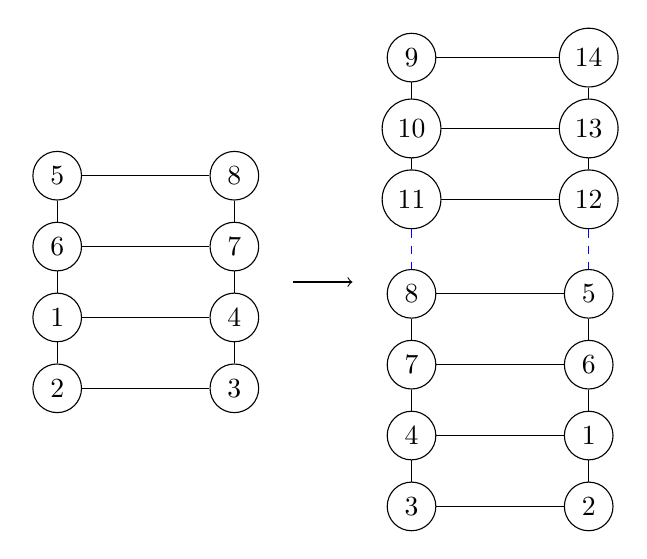
\begin{tikzpicture}[x=.75cm, y=.75cm]
				\fill[nearly opaque, white] (-2, -3.5) rectangle (8, 3);
				\begin{scope}[circle, minimum size=15pt, every node/.style=draw]
					\node (1) at (-1.5, 1.8) {5};
					\node (2) at (-1.5, 0.6) {6};
					\node (3) at (-1.5, -0.6) {1};
					\node (4) at (-1.5, -1.8) {2};
					\node (5) at (1.5, -1.8) {3};
					\node (6) at (1.5, -0.6) {4};
					\node (7) at (1.5, 0.6) {7};
					\node (8) at (1.5, 1.8) {8};
				\end{scope}
				\path (1) edge (2) edge (8);
				\path (2) edge (3) edge (7);
				\path (3) edge (4) edge (6);
				\path (4) edge (5);
				\path (5) edge (6);
				\path (6) edge (7);
				\path (7) edge (8);
				\draw[->] (2.5, 0) -- (3.5, 0);
				\begin{scope}[shift={(6, 0)}, circle, minimum size=15pt, every node/.style=draw]
					\node (1) at (-1.5, 3.8) {9};
					\node (2) at (-1.5, 2.6) {10};
					\node (3) at (-1.5, 1.4) {11};
					\node (4) at (-1.5, -0.2) {8};
					\node (5) at (-1.5, -1.4) {7};
					\node (6) at (-1.5, -2.6) {4};
					\node (7) at (-1.5, -3.8) {3};
					\node (8) at (1.5, -3.8) {2};
					\node (9) at (1.5, -2.6) {1};
					\node (10) at (1.5, -1.4) {6};
					\node (11) at (1.5, -0.2) {5};
					\node (12) at (1.5, 1.4) {12};
					\node (13) at (1.5, 2.6) {13};
					\node (14) at (1.5, 3.8) {14};
				\end{scope}
				\path (1) edge (2) edge (14);
				\path (2) edge (3) edge (13);
				\path (3) edge [dashed, blue] (4) edge (12);
				\path (4) edge (5) edge (11);
				\path (5) edge (6) edge (10);
				\path (6) edge (7) edge (9);
				\path (7) edge (8);
				\path (8) edge (9);
				\path (9) edge (10);
				\path (10) edge (11);
				\path (12) edge [dashed, blue] (11) edge (13);
				\path (13) edge (14);
			\end{tikzpicture}
			\caption{}
		\end{figure}
	}{
		是否有 $L_n \subseteq H_{2 n}$?

		\onslide<2->{如果 $2 n + 1$ 是素数,那么容易构造。}

		\onslide<3->{否则?取正奇数 $2 k + 1$ 使得 $2 n + 2 k + 1$ 是素数,然后将梯子搭到 $(n + k, n + k + 1)$。}

		\onslide<4->{\textsl{如果这个梯子和 $2 k$ 时构造的梯子相容},那么,就完成了 $2 n$ 时的构造。}
	}
}

\sol {
	这样的构造一定存在吗?如果存在,怎样快速寻找?\pause

	其实很简单,\emm{\textsl{我们不需要证明对任意 $n$ 存在,我们只需要证明对 $n \leq 2 \times 10^5$ 存在}},这样只需用程序暴力验证一下对于每个 $2 n$ 的最小解 $c(2 n)$。\pause

	经验证知 $\sum\limits_{n=1}^{10^5} c(2 n) = 1\,272\,400$,因此可以接受。\pause

	对于一般图的情形,要注意 $1$ 可能会分配给 1 度点之间的连边,因此实际实现的时候我们是对 $2 \sim 2 n + 1$ 进行``搭梯子''。
}
